\providecommand{\main}{../../../..}
\documentclass[\main/dresen_thesis.tex]{subfiles}
\begin{document}
  \label{sec:colloidalCrystals:nanoparticle:vsm}
  \begin{figure}[tb]
    \centering
    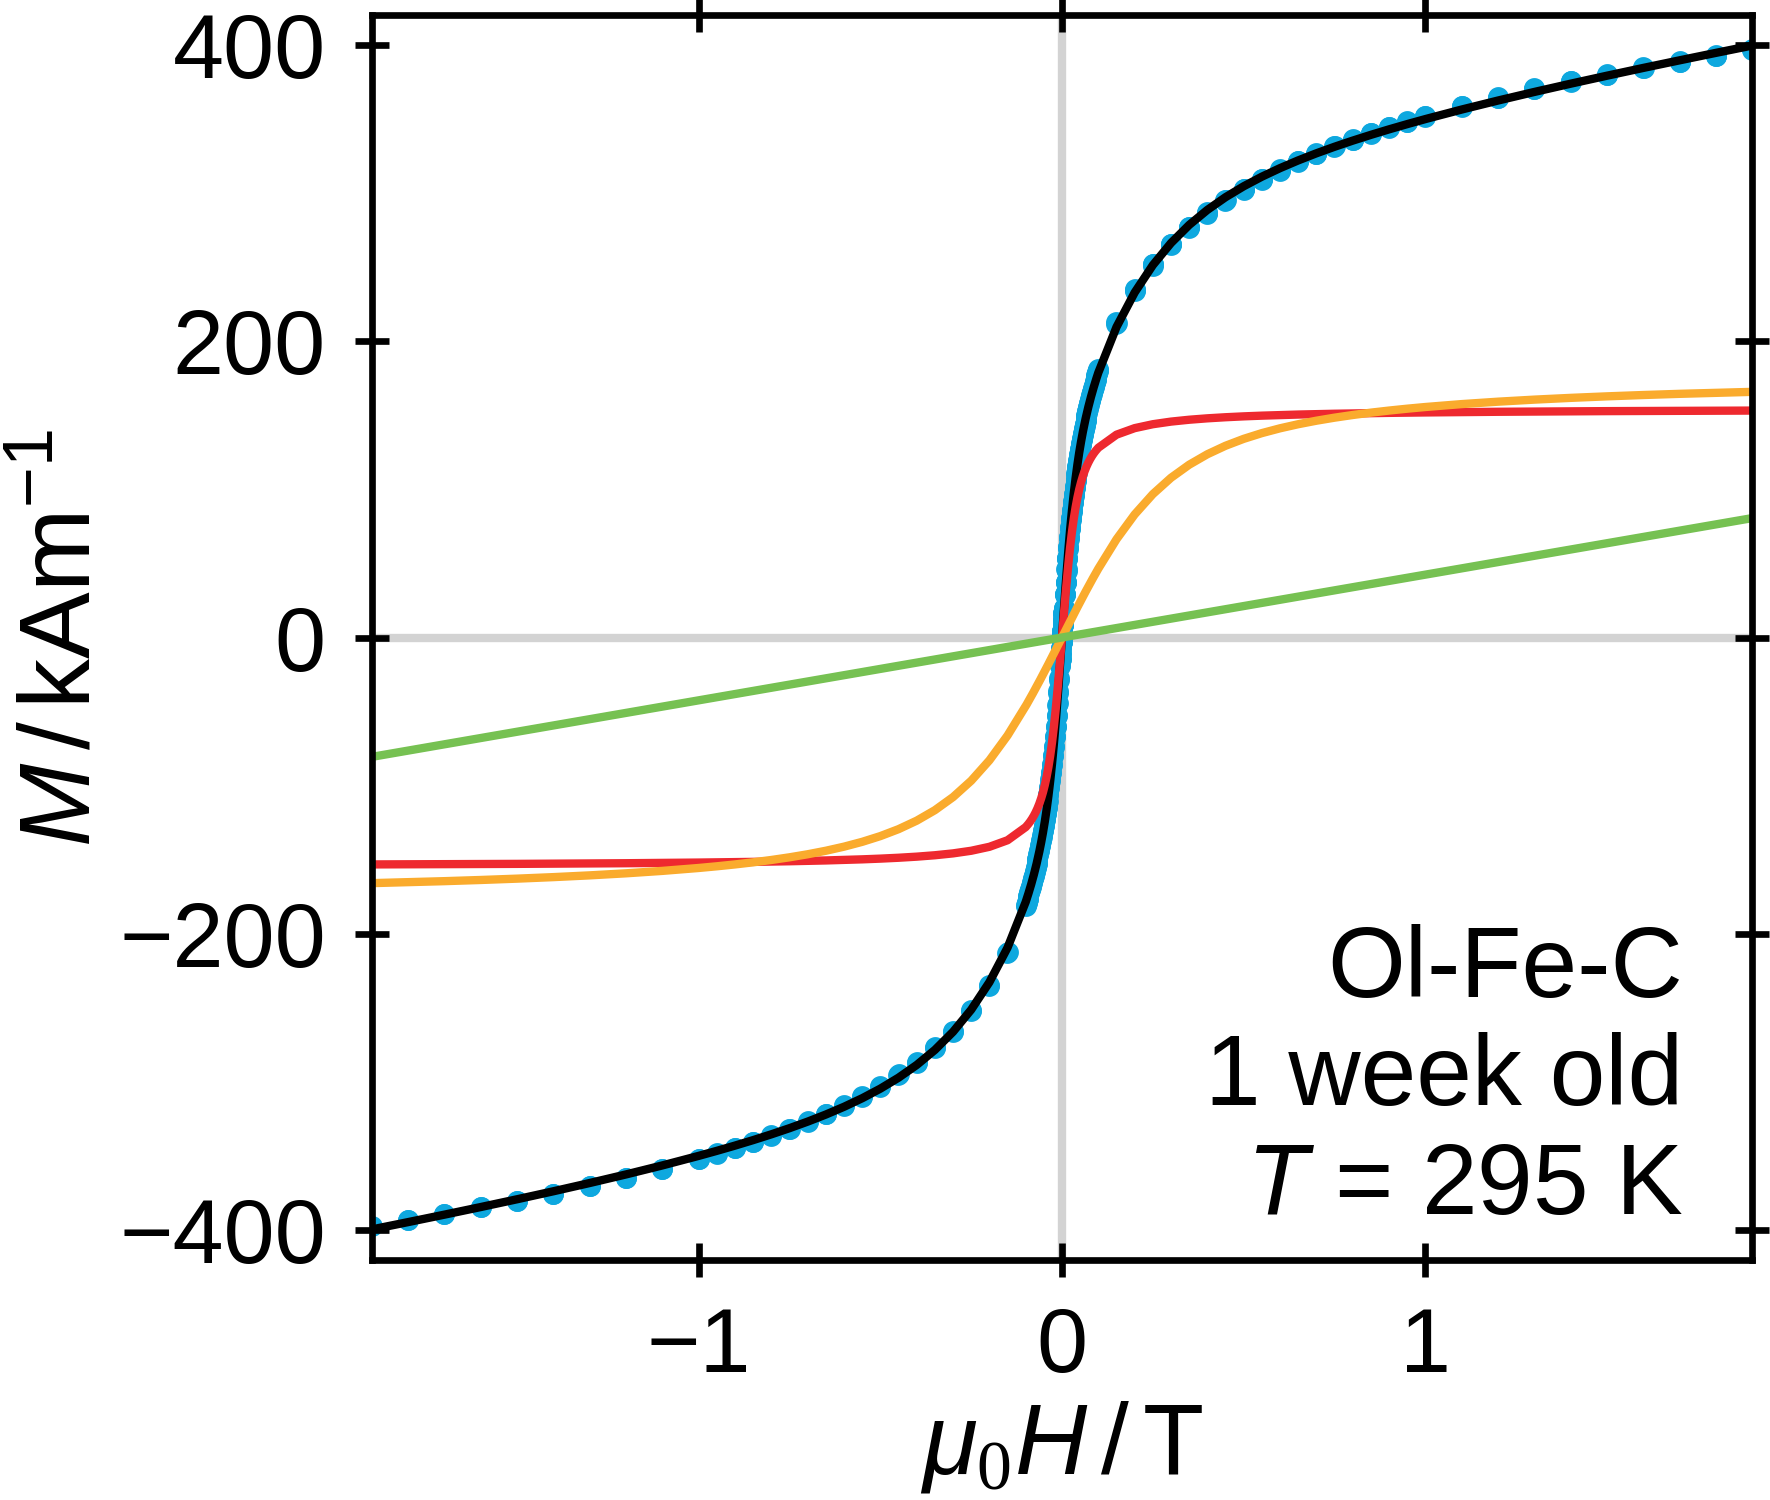
\includegraphics{colloidalCrystals_VSM_Ol_Fe_C}
    \caption{\label{fig:colloidalCrystals:nanoparticle:vsm}Room temperature VSM of Ol-Fe-C performed on a dry powder right after nanocube synthesis.}
  \end{figure}
  The magnetization of the nanocubes in a dry powder is shown in \reffig{fig:colloidalCrystals:nanoparticle:vsm} as measured within the week after synthesis.
  The obtained data from the powder deviates from a typical Langevin behaviour with excess susceptibility, as to why a linear combination of two Langevin behaviour and excess susceptibility is used to properly describe the data.
  The parameters before rescaling of the data from the best fit obtained by this model are tabulated in \reftab{tab:colloidalCrystals:nanoparticle:vsm}.

  \begin{table}[!htbp]
    \centering
    \caption{\label{tab:colloidalCrystals:nanoparticle:vsm} Fit parameters determined from the field-dependent magnetization measurements of the dried nanocubes at room temperature. A linear combination of two Langevin behaviour is fit, where $\mu_i$ is the single-particle magnetic moment and $\tilde{M}_{s,\,i}$ the spontaneous magnetization and $i\eq 1,\,2$ the two modes. $\tilde{\chi}$ is an additional excess susceptibility. The parameters are given in the units as measured from VSM. The parameters $M_{s,\,i}$ and $\chi$ scaled to the magnetic volume are determined as described in the text.}
    \begin{tabular}{ l | l }
      \rule{0pt}{2ex} \textbf{VSM @ 295 K} & Linear Comb. of Two Langevin \\
      \hline
      \rule{0pt}{2ex} $\mu_1 \, / \, \mu_B$                     & $25600(264)$\\
      \rule{0pt}{2ex} $\mu_2 \, / \, \mu_B$                     & $3605(65) $ \\
      \rule{0pt}{2ex} $\tilde{M}_{s,\,1} \, /  \unit{memu}$     & $11.3(1)$    \\
      \rule{0pt}{2ex} $\tilde{M}_{s,\,2} \, /  \unit{memu}$     & $13.0(1)$    \\
      \rule{0pt}{2ex} $\tilde{\chi} \, / \unit{memu \, T^{-1}}$ & $3.12(5)$\\
      \hline
      \rule{0pt}{2ex} $M_{s,\,1} \, /  \unit{kA\,m^{-1}}$       & $155(1)$    \\
      \rule{0pt}{2ex} $M_{s,\,2} \, /  \unit{kA\,m^{-1}}$       & $177(1)$    \\
      \rule{0pt}{2ex} $\mu_0 \chi \, / \, 10^{-6}$              & $53300(900)$\\
      \hline
    \end{tabular}
  \end{table}

  A magnetic moment of $25600(264) \mu_B$ is determined for the first mode and a smaller moment of $3605(65) \mu_B$ for the second mode.
  From the magnetic moment and the determined spontaneous magnetizations, the number of moments in the separate modes is determined to $N_1 \eq 47.7 \cdot 10^{12}$ and $N_2 \eq 388 \cdot 10^{12}$.
  Estimating the magnetic volume from the first mode and the particle volume from small-angle scattering in \refsec{sec:colloidalCrystals:nanoparticle:sas} a value of $V_\mathrm{mag} \eq N_1 V_p \eq 0.074 \unit{\musf L}$ or a mass of $0.38 \unit{mg}$ if a particle density of $5.2 \unit{g \, mL^{-1}}$ is estimated.
  This is in a similar order of magnitude ($\approx 50\%$) as roughly estimated from gravimetrically determining the particle concentration of the stock solution and the amount of solvent transferred to the measurement container.
  The smaller value suggests, that either the concentration of the stock solution is overestimated as not everything that is measured gravimetrically corresponds to the magnetic material but also contains organic contents, or that by the estimate of $N\eq N_1$ the total magnetic volume is slightly underestimated.
  In each case this means that the determined rescaled magnetizations are an upper limit for the true volume magnetization of the sample.
  Rescaling the data to the determined magnetic volume $V_\mathrm{mag}$, the values $M_{s,\,1}$, $M_{s,\,2}$ and $\chi$ are obtained as tabulated in \reftab{tab:colloidalCrystals:nanoparticle:vsm}.

  The first mode corresponds to a spontaneous magnetization of $155(1) \unit{kA \, m^{-1}}$ and the second mode has a spontaneous magnetization in a similar order of magnitude with $177(1) \unit{kA \, m^{-1}}$.
  The excess susceptibility is unusually large with an order of magnitude of $\mu_0 \chi \eq 53300(900) \cdot 10^{-6}$.
  A purely w\"ustite contribution would be expected at ambient conditions in the order of $7230 \cdot 10^{-6}$ \cite{Lide_2004_Handb}.
  One possibility for this is that the $\pm 2 \unit{T}$ range is not sufficient to properly determine the slope of the excess susceptibility, which results in this systematic error.
  The two determined spontaneous magnetizations are significantly smaller than bulk magnetite ($M_\mathrm{magnetite} \eq 475 - 517 \unit{kA \, m^{-1}}$ \cite{Cornell_2003_Their, Handley_2000_Moder}) and also smaller than the value that is observed by later performed SANSPOL experiment in \refsec{sec:colloidalCrystals:nanoparticle:sas}.
  This is to be understood for one by the chronologically placement of the experiment early on right after the synthesis, where the oxidation process of the nanoparticle is in an early stage and a large fraction of the nanoparticle is in a w\"ustite phase.
  For the other, the stated spontaneous magnetization are to be considered for the primary mode as if the moments is distributed over the whole particle volume $V_p$, as effectively $M_{s,\,1} \eq \mu_1 / V_p$ is calculated.
  For the second mode $M_{s,\,2} \eq N_2 \mu_2 / (N_1 V_p)$ is calculated, which corresponds to $N_2/N_1$ moments distributed on each particle of volume $V_p$.
  However, $\mu_1$ are supposedly parts of the magnetic shell of the nanocubes and therefore only smaller volumes should actually be considered when stating the spontaneous magnetization of the material, which results in the observed discrepancy.

  From the limited information given by VSM, it is not straight forward to correct the discrepancy.
  Furthermore, it has to be said that the performed VSM measurements are sub-optimal to characterize the non-interacting nanocube properties, as for one they were performed for a dry sample and thus likely affected by interparticle interactions.
  From the unstable phase of the nanocubes, it is difficult to compare the results across multiple complimentary experiments.
  An improved VSM study using nanocubes in a well-defined phase and within a well-diluted state is however not performed as part of this thesis.
\end{document}
